\documentclass{standalone}
\usepackage{tikz}
\usetikzlibrary{patterns, positioning}
\usepackage[sfdefault]{ClearSans} %% option 'sfdefault' activates Clear Sans as the default text font
\usepackage[T1]{fontenc}

\begin{document}
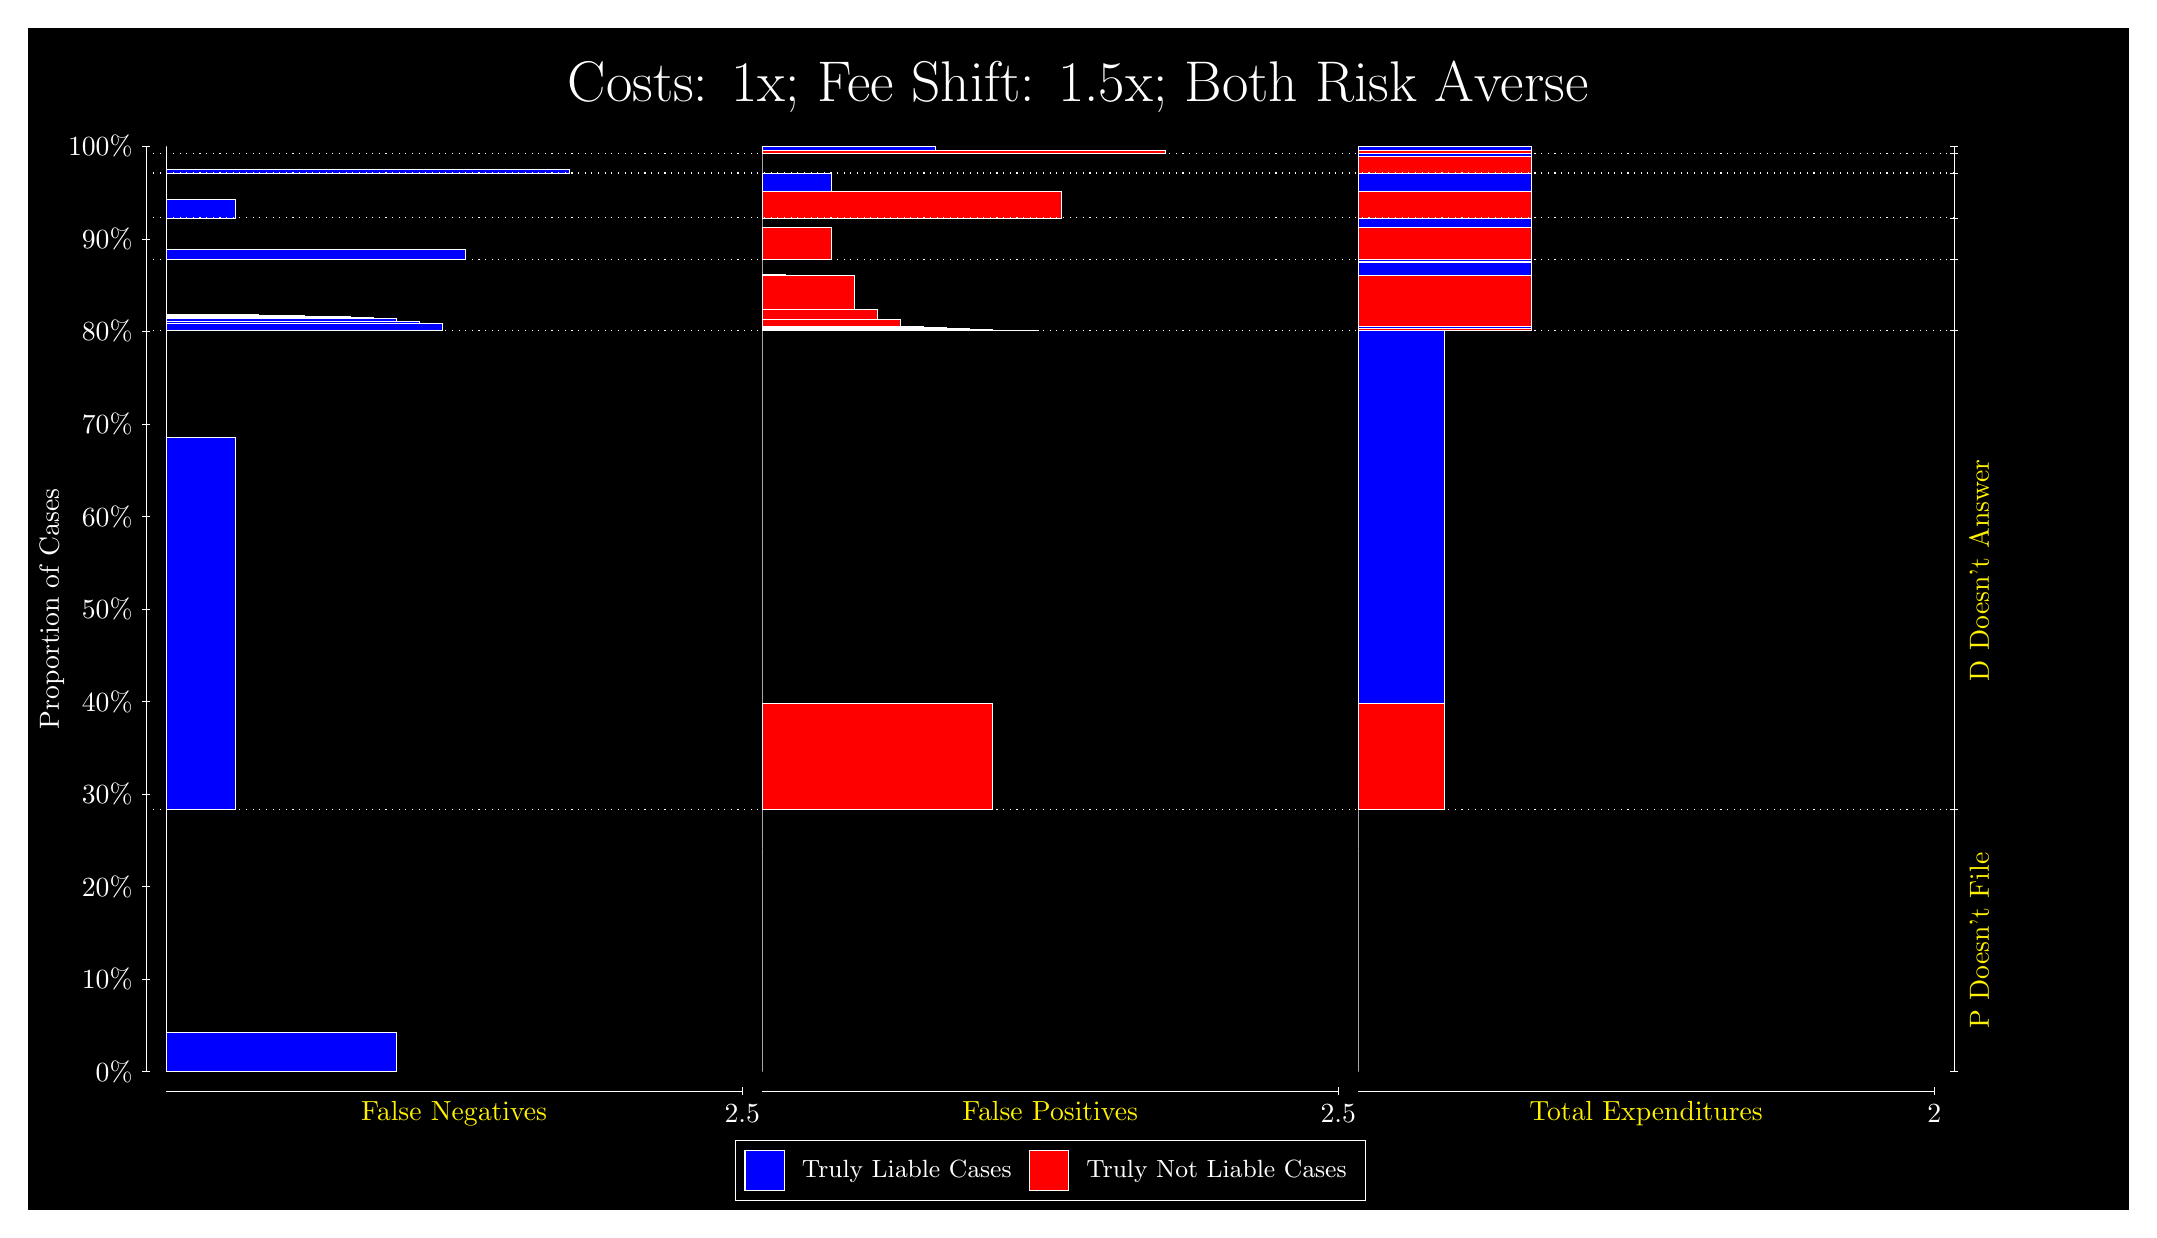
\begin{tikzpicture}
\draw[fill=black] (0,0) rectangle (26.667,15);
\draw[text=white] (0,13.5) rectangle (26.667,15) node[midway] {\huge Costs: 1x; Fee Shift: 1.5x; Both Risk Averse};
\draw[white, very thin] (1.5,1.75) -- (1.5,13.5);
\node[rotate=90, text=white, anchor=center] at (0.3, 7.625) {Proportion of Cases};
\draw[white, very thin] (1.45,1.75) -- (1.55,1.75);
\node[text=white, anchor=east] at (1.45, 1.75) {0\%};
\draw[white, very thin] (1.45,2.925) -- (1.55,2.925);
\node[text=white, anchor=east] at (1.45, 2.925) {10\%};
\draw[white, very thin] (1.45,4.1) -- (1.55,4.1);
\node[text=white, anchor=east] at (1.45, 4.1) {20\%};
\draw[white, very thin] (1.45,5.275) -- (1.55,5.275);
\node[text=white, anchor=east] at (1.45, 5.275) {30\%};
\draw[white, very thin] (1.45,6.45) -- (1.55,6.45);
\node[text=white, anchor=east] at (1.45, 6.45) {40\%};
\draw[white, very thin] (1.45,7.625) -- (1.55,7.625);
\node[text=white, anchor=east] at (1.45, 7.625) {50\%};
\draw[white, very thin] (1.45,8.8) -- (1.55,8.8);
\node[text=white, anchor=east] at (1.45, 8.8) {60\%};
\draw[white, very thin] (1.45,9.975) -- (1.55,9.975);
\node[text=white, anchor=east] at (1.45, 9.975) {70\%};
\draw[white, very thin] (1.45,11.15) -- (1.55,11.15);
\node[text=white, anchor=east] at (1.45, 11.15) {80\%};
\draw[white, very thin] (1.45,12.325) -- (1.55,12.325);
\node[text=white, anchor=east] at (1.45, 12.325) {90\%};
\draw[white, very thin] (1.45,13.5) -- (1.55,13.5);
\node[text=white, anchor=east] at (1.45, 13.5) {100\%};

\draw[white, very thin] (24.457,1.75) -- (24.457,13.5);
\draw[white, very thin] (24.407,1.75) -- (24.507,1.75);
\node[anchor=west] at (24.407, 1.75) {};
\draw[white, very thin] (24.407,5.0772) -- (24.507,5.0772);
\node[anchor=west] at (24.407, 5.0772) {};
\draw[white, very thin] (24.407,11.159) -- (24.507,11.159);
\node[anchor=west] at (24.407, 11.159) {};
\draw[white, very thin] (24.407,12.063) -- (24.507,12.063);
\node[anchor=west] at (24.407, 12.063) {};
\draw[white, very thin] (24.407,12.591) -- (24.507,12.591);
\node[anchor=west] at (24.407, 12.591) {};
\draw[white, very thin] (24.407,13.161) -- (24.507,13.161);
\node[anchor=west] at (24.407, 13.161) {};
\draw[white, very thin] (24.407,13.412) -- (24.507,13.412);
\node[anchor=west] at (24.407, 13.412) {};
\draw[white, very thin] (24.407,13.5) -- (24.507,13.5);
\node[anchor=west] at (24.407, 13.5) {};

\draw[white, very thin, fill=blue] (1.75,1.75) rectangle (4.6775,2.2433);
\draw[white, very thin, fill=red] (1.75,2.2433) rectangle (1.75,5.0772);
\draw[white, very thin, fill=blue] (1.75,5.0772) rectangle (2.6283,9.8035);
\draw[white, very thin, fill=red] (1.75,9.8035) rectangle (1.75,11.159);
\draw[white, very thin, fill=blue] (1.75,11.159) rectangle (5.2631,11.247);
\draw[white, very thin, fill=blue] (1.75,11.247) rectangle (4.9703,11.284);
\draw[white, very thin, fill=blue] (1.75,11.284) rectangle (4.6775,11.321);
\draw[white, very thin, fill=blue] (1.75,11.321) rectangle (4.3848,11.324);
\draw[white, very thin, fill=blue] (1.75,11.324) rectangle (4.3848,11.33);
\draw[white, very thin, fill=blue] (1.75,11.33) rectangle (4.092,11.341);
\draw[white, very thin, fill=blue] (1.75,11.341) rectangle (3.7993,11.347);
\draw[white, very thin, fill=blue] (1.75,11.347) rectangle (3.5065,11.353);
\draw[white, very thin, fill=blue] (1.75,11.353) rectangle (3.2138,11.357);
\draw[white, very thin, fill=blue] (1.75,11.357) rectangle (2.921,11.364);
\draw[white, very thin, fill=red] (1.75,11.364) rectangle (1.75,12.063);
\draw[white, very thin, fill=blue] (1.75,12.063) rectangle (5.5558,12.187);
\draw[white, very thin, fill=red] (1.75,12.187) rectangle (1.75,12.591);
\draw[white, very thin, fill=blue] (1.75,12.591) rectangle (2.6283,12.828);
\draw[white, very thin, fill=red] (1.75,12.828) rectangle (1.75,13.161);
\draw[white, very thin, fill=blue] (1.75,13.161) rectangle (6.8732,13.203);
\draw[white, very thin, fill=red] (1.75,13.203) rectangle (1.75,13.412);
\draw[white, very thin, fill=red] (1.75,13.412) rectangle (1.75,13.454);
\draw[white, very thin, fill=blue] (1.75,13.454) rectangle (1.75,13.5);
\draw[white, very thin, fill=red] (9.3189,1.75) rectangle (9.3189,4.584);
\draw[white, very thin, fill=blue] (9.3189,4.584) rectangle (9.3189,5.0772);
\draw[white, very thin, fill=red] (9.3189,5.0772) rectangle (12.246,6.4325);
\draw[white, very thin, fill=blue] (9.3189,6.4325) rectangle (9.3189,11.159);
\draw[white, very thin, fill=red] (9.3189,11.159) rectangle (12.832,11.163);
\draw[white, very thin, fill=red] (9.3189,11.163) rectangle (12.539,11.167);
\draw[white, very thin, fill=red] (9.3189,11.167) rectangle (12.246,11.175);
\draw[white, very thin, fill=red] (9.3189,11.175) rectangle (11.954,11.185);
\draw[white, very thin, fill=red] (9.3189,11.185) rectangle (11.661,11.203);
\draw[white, very thin, fill=red] (9.3189,11.203) rectangle (11.368,11.219);
\draw[white, very thin, fill=red] (9.3189,11.219) rectangle (11.075,11.305);
\draw[white, very thin, fill=red] (9.3189,11.305) rectangle (10.783,11.425);
\draw[white, very thin, fill=red] (9.3189,11.425) rectangle (10.49,11.858);
\draw[white, very thin, fill=blue] (9.3189,11.858) rectangle (9.9044,11.865);
\draw[white, very thin, fill=blue] (9.3189,11.865) rectangle (9.6116,11.869);
\draw[white, very thin, fill=blue] (9.3189,11.869) rectangle (9.3189,12.063);
\draw[white, very thin, fill=red] (9.3189,12.063) rectangle (10.197,12.467);
\draw[white, very thin, fill=blue] (9.3189,12.467) rectangle (9.3189,12.591);
\draw[white, very thin, fill=red] (9.3189,12.591) rectangle (13.125,12.923);
\draw[white, very thin, fill=blue] (9.3189,12.923) rectangle (10.197,13.161);
\draw[white, very thin, fill=red] (9.3189,13.161) rectangle (9.3189,13.37);
\draw[white, very thin, fill=blue] (9.3189,13.37) rectangle (9.3189,13.412);
\draw[white, very thin, fill=red] (9.3189,13.412) rectangle (14.442,13.454);
\draw[white, very thin, fill=blue] (9.3189,13.454) rectangle (11.515,13.5);
\draw[white, very thin, fill=red] (16.888,1.75) rectangle (16.888,4.584);
\draw[white, very thin, fill=blue] (16.888,4.584) rectangle (16.888,5.0772);
\draw[white, very thin, fill=red] (16.888,5.0772) rectangle (17.986,6.4325);
\draw[white, very thin, fill=blue] (16.888,6.4325) rectangle (17.986,11.159);
\draw[white, very thin, fill=red] (16.888,11.159) rectangle (19.083,11.19);
\draw[white, very thin, fill=blue] (16.888,11.19) rectangle (19.083,11.211);
\draw[white, very thin, fill=red] (16.888,11.211) rectangle (19.083,11.858);
\draw[white, very thin, fill=blue] (16.888,11.858) rectangle (19.083,12.024);
\draw[white, very thin, fill=red] (16.888,12.024) rectangle (19.083,12.045);
\draw[white, very thin, fill=blue] (16.888,12.045) rectangle (19.083,12.063);
\draw[white, very thin, fill=red] (16.888,12.063) rectangle (19.083,12.467);
\draw[white, very thin, fill=blue] (16.888,12.467) rectangle (19.083,12.591);
\draw[white, very thin, fill=red] (16.888,12.591) rectangle (19.083,12.923);
\draw[white, very thin, fill=blue] (16.888,12.923) rectangle (19.083,13.161);
\draw[white, very thin, fill=red] (16.888,13.161) rectangle (19.083,13.37);
\draw[white, very thin, fill=blue] (16.888,13.37) rectangle (19.083,13.412);
\draw[white, very thin, fill=red] (16.888,13.412) rectangle (19.083,13.454);
\draw[white, very thin, fill=blue] (16.888,13.454) rectangle (19.083,13.5);
\draw[white, dotted] (1.5,5.0772) -- (24.457,5.0772);
\draw[white, dotted] (1.5,11.159) -- (24.457,11.159);
\draw[white, dotted] (1.5,12.063) -- (24.457,12.063);
\draw[white, dotted] (1.5,12.591) -- (24.457,12.591);
\draw[white, dotted] (1.5,13.161) -- (24.457,13.161);
\draw[white, dotted] (1.5,13.412) -- (24.457,13.412);
\draw[white, very thin] (1.75,1.5) -- (9.0689,1.5);
\node[text=yellow, anchor=north] at (5.4094, 1.5) {False Negatives};
\draw[white, very thin] (9.0689,1.45) -- (9.0689,1.55);
\node[text=white, anchor=north] at (9.0689, 1.45) {2.5};

\draw[white, very thin] (9.3189,1.5) -- (16.638,1.5);
\node[text=yellow, anchor=north] at (12.978, 1.5) {False Positives};
\draw[white, very thin] (16.638,1.45) -- (16.638,1.55);
\node[text=white, anchor=north] at (16.638, 1.45) {2.5};

\draw[white, very thin] (16.888,1.5) -- (24.207,1.5);
\node[text=yellow, anchor=north] at (20.547, 1.5) {Total Expenditures};
\draw[white, very thin] (24.207,1.45) -- (24.207,1.55);
\node[text=white, anchor=north] at (24.207, 1.45) {2};

\node[text=yellow, centered, rotate=90] at (24.777, 3.4136) {P Doesn't File};
\node[text=yellow, centered, rotate=90] at (24.777, 8.118) {D Doesn't Answer};






\draw (12.978300999999998,1.5) node[draw=none] (baseCoordinate) {};
\begin{scope}[align=center]
        \matrix[scale=0.5, draw=white, below=0.5cm of baseCoordinate, nodes={draw}, column sep=0.1cm]{
            \node[rectangle, draw, minimum width=0.5cm, minimum height=0.5cm, fill=blue] {}; &
            \node[draw=none, font=\small, text=white] (B) {Truly Liable Cases}; &
            \node[rectangle, draw, minimum width=0.5cm, minimum height=0.5cm, fill=red] {}; &
            \node[draw=none, font=\small, text=white] (B) {Truly Not Liable Cases}; \\
            };
\end{scope}

\end{tikzpicture}
\end{document}